% Provenance (never printed): old terminale S material on the Earth's internal
% heat (geothermal gradient and heat flow, radioactive heat production,
% conduction and convection, mantle convection, geothermal energy). Owner
% (Sync 0/1): heat flow, radiogenic heat production, secular cooling, thermal
% and mantle convection (recall the convection cell of Book 1 g8 first),
% geothermal energy. Geotherm and geothermal gradient are g11.03's; radioactivity,
% half-life, decay law and thermal conductivity are physics' (thermal
% conductivity used as "the rock's thermal conductivity k", never defined);
% hotspot track and plume g11.04's. Figures: figdata/grade-12/internal_heat.py.
\chapter{पृथ्वी की आंतरिक ऊष्मा}\label{ch:g12:internal-heat}

1987 और 1995 के बीच, बवेरिया में विंडिशेशेनबाख गाँव के निकट,
भूवैज्ञानिकों ने \omterm{def:g12:continental-crust:continental-crust}{महाद्वीपीय भूपर्पटी} में \qty{9101}{m} गहरा एक छेद खोदा। तली पर
चट्टान लगभग \qty{265}{\celsius} पर थी, इतनी गरम कि और गहरा खोदना
संभव नहीं था।
% ledger: gfz:ktb, gfz:ktb30

सतह पर लगभग \qty{10}{\celsius} से \qty{9.1}{km} पर \qty{265}{\celsius} तक की
वृद्धि प्रति किलोमीटर लगभग \qty{28}{\celsius} है, एक सामान्य
मान। पृथ्वी पर हर जगह नीचे की ओर गरमी बढ़ती है, इसलिए ऊष्मा
पृथ्वी से लगातार बाहर बहती है। यह अध्याय उस प्रवाह को मापता है, पूछता है कि ऊष्मा
कहाँ से आती है, और दिखाता है कि वह कैसे चलती है।
% values: ktb_gradient 28.0 (internal_heat.py, surface temperature taken as 10 degC); ledger: gfz:ktb (gradient about 28 K/km)

\begin{recall}
\omterm{def:g11:lithosphere-asthenosphere:geotherm}{भूतापीय वक्र} किसी स्थान के नीचे गहराई के सापेक्ष तापमान का वक्र है, और
\omterm{def:g11:lithosphere-asthenosphere:geotherm}{भूतापीय प्रवणता} प्रति किलोमीटर तापमान की वृद्धि; बोरछिद्र
सतह के निकट प्रति किलोमीटर 25 से \qty{30}{\celsius} मापते हैं
(\cref{ch:g11:lithosphere-asthenosphere})। कुछ परमाणु रेडियोधर्मी होते हैं: वे
यादृच्छिक रूप से क्षयित होते हैं, बचे हुए परमाणुओं की संख्या हर अर्ध-आयु में आधी होती जाती है, और हर
क्षय ऊर्जा मुक्त करता है, जो अंत में ऊष्मा बन जाती है (भौतिकी की पुस्तकें)।
संवहन कोष्ठ तरल का एक लूप है जो नीचे से गरम होता है, ऊपर उठता है, फैलता है,
ठंडा होता है और डूबता है (पुस्तक 1, कक्षा 8)। तप्त स्थल पर कोई प्लेट गरम प्रावार के
एक प्लूम के ऊपर से चलती है (\cref{ch:g11:plate-motions})।
\end{recall}
% ledger: usgs:gradient-29 (Book 1 row)

\section{प्रवणता और ऊष्मा-प्रवाह}

\begin{definition}[ऊष्मा-प्रवाह]\label{def:g12:internal-heat:heat-flow}
किसी स्थान पर \emph{ऊष्मा-प्रवाह}\index{ऊष्मा-प्रवाह} (या ऊष्मा-फ़्लक्स) वह
शक्ति है जो वहाँ पृथ्वी के भीतरी भाग से उसकी सतह के हर वर्ग मीटर से होकर
निकलती है। इसे मिलीवाट प्रति वर्ग मीटर
(\unit{mW/m^2}) में मापा जाता है।
\end{definition}
% ledger: b2dd10:continents

ऊष्मा गरम से ठंडे की ओर बहती है, और तापमान-प्रवणता जितनी तीव्र, वह उतनी ही
तेज़ी से बहती है। कितनी बहती है, यह चट्टान पर भी निर्भर है: हर चट्टान की एक
ऊष्मा-चालकता $k$ होती है, वाट प्रति मीटर प्रति केल्विन में, जिसे भौतिकी की
पुस्तकें परिभाषित करती हैं।

\begin{proposition}[ऊष्मा-प्रवाह और प्रवणता]\label{prop:g12:internal-heat:fourier}
ऊष्मा-चालकता $k$ वाली ऐसी चट्टान से होकर, जिसमें तापमान गहराई के साथ
प्रवणता $G$ (केल्विन प्रति मीटर में) से बढ़ता है, सतह की ओर ऊपर
\omterm{def:g12:internal-heat:heat-flow}{ऊष्मा-प्रवाह} है
\[
  q = k\,G .
\]
\end{proposition}

चालन का यह नियम, जो फ़ूरिए का है, यहाँ मान लिया गया है; भौतिकी की पुस्तकें
इसे एक व्यापक रूप में सिद्ध करती हैं।

\begin{method}[बोरछिद्र से ऊष्मा-प्रवाह]\label{met:g12:internal-heat:borehole}
\begin{enumerate}
  \item किसी बोरछिद्र की कई गहराइयों पर तापमान मापिए, जब
        छिद्र को चट्टान के तापमान पर लौटने का समय मिल चुका हो।
  \item गहराई के सापेक्ष तापमान आलेखित कीजिए और ढाल लीजिए: प्रवणता $G$,
        केल्विन प्रति मीटर में बदली हुई।
  \item प्रयोगशाला में कोरों पर चट्टान की चालकता $k$
        मापिए।
  \item गुणा कीजिए: $q = kG$, \unit{W/m^2} में, फिर \unit{mW/m^2} में बदलिए।
\end{enumerate}
\end{method}

\begin{example}[ग्रेनाइट में एक बोरछिद्र]\label{ex:g12:internal-heat:borehole}
\qty{2.72}{W/(m.K)} चालकता वाले ग्रेनाइट में एक बोरछिद्र
प्रति किलोमीटर \qty{29}{\celsius} की प्रवणता मापता है, यानी \qty{0.029}{K/m}।
तब $q = 2.72 \times 0.029 \approx \qty{0.079}{W/m^2}$, लगभग
\qty{79}{mW/m^2}।
\end{example}
% ledger: roy:conductivity (granitic layer 6.5 mcal/(cm s degC) = 2.72 W/m/K), usgs:gradient-29 (Book 1 row)
% values: borehole_q_mW 78.9 (internal_heat.py)

ऐसे 38\,000 से अधिक मापनों को मिलाकर पूरी पृथ्वी का एक मानचित्र
बनाया गया है। महाद्वीप औसतन \qty{70.9}{mW/m^2} खोते हैं, महासागरीय
तली \qty{105.4}{mW/m^2}; पूरी सतह पर \qty{91.6}{mW/m^2}।
पृथ्वी के क्षेत्रफल, \qty{5.101e14}{m^2}, से गुणा करने पर कुल यह है:
\[
  0.0916 \times \num{5.101e14} \approx \qty{4.67e13}{W} = \qty{46.7}{TW},
\]
लगभग 47 टेरावाट, 2 कम या अधिक।
% ledger: b2dd10:continents, b2dd10:half-space (47 +- 2 TW, 38,347 measurements)

महासागरीय तली वहाँ सबसे अधिक खोती है जहाँ वह सबसे नई है। नया \omterm{def:g11:lithosphere-asthenosphere:lithosphere}{स्थलमंडल} किसी
कटक से गरम निकलता है, और दूर जाते हुए ठंडा होता है; उसका \omterm{def:g12:internal-heat:heat-flow}{ऊष्मा-प्रवाह} उसकी
आयु के वर्गमूल के व्युत्क्रम के अनुपात में गिरता है।

\begin{omfigure}
\begin{tikzpicture}
\begin{axis}[omrecord, width=0.72\linewidth, height=5.6cm, xmin=0, xmax=180, ymin=0, ymax=400,
  xlabel={महासागरीय तली की आयु (मिलियन वर्ष)}, ylabel={ऊष्मा-प्रवाह (\unit{mW/m^2})},
  xtick={0,30,...,180}, ytick={0,100,...,400}]
% computed in figdata/grade-12/internal_heat.py; ledger: b2dd10:half-space, b2dd10:continents
\addplot[omDef, line width=1.1pt, restrict x to domain=0:66.5] table[x=t_Myr, y=q] {figdata/out/grade-12-internal_heat-halfspace.dat};
\addplot[omDef, line width=1.1pt, densely dotted, restrict x to domain=66.5:180] table[x=t_Myr, y=q] {figdata/out/grade-12-internal_heat-halfspace.dat};
\addplot[omProp, line width=0.9pt, dashed, domain=0:180] {70.9};
\coordinate (lawlab) at (axis cs:14,250);
\coordinate (contlab) at (axis cs:100,80);
\end{axis}
\node[font=\scriptsize, text=omDef, anchor=west] at (lawlab) {$q = 490/\sqrt{t}$};
\node[font=\scriptsize, text=omProp, anchor=south west] at (contlab) {महाद्वीपों का माध्य, \qty{70.9}{mW/m^2}};
\end{tikzpicture}

{\small महासागरीय तली से होकर \omterm{def:g12:internal-heat:heat-flow}{ऊष्मा-प्रवाह}, उसकी आयु के सापेक्ष, जैसा
\omterm{def:g11:lithosphere-asthenosphere:lithosphere}{स्थलमंडल} के ठंडे होने के लिए परिकलित किया गया है ($t$ मिलियन वर्षों में); 66.5
मिलियन वर्ष के आगे (बिंदुकित) यह नियम कम ठीक बैठता है। स्रोत: डेविस
और डेविस (2010)।}
\end{omfigure}
% values: q_1Myr 490, q_10Myr 155, q_66.5Myr 60.1, age_where_q_equals_cont_Myr 47.8 (internal_heat.py)

\section{ऊष्मा कहाँ से आती है}

ऊष्मा के दो स्रोत हैं। पहला रेडियोधर्मिता है।

\begin{definition}[रेडियोजनित ऊष्मा-उत्पादन]\label{def:g12:internal-heat:heat-production}
किसी चट्टान का \emph{रेडियोजनित ऊष्मा-उत्पादन}\index{रेडियोजनित ऊष्मा-उत्पादन}
वह ऊष्मा है जो उसके भीतर उसके रेडियोधर्मी परमाणुओं के क्षय से मुक्त होती है,
प्रति इकाई आयतन और समय, माइक्रोवाट प्रति घन मीटर में
(\unit{\micro W/m^3})। इसका लगभग सारा भाग चार समस्थानिकों से आता है: यूरेनियम-238,
यूरेनियम-235, थोरियम-232 और पोटैशियम-40।
\end{definition}
% ledger: dye12:isotopes, earle:heat-sources, kamland11:geonu

ये तत्त्व \omterm{def:g12:continental-crust:continental-crust}{महाद्वीपीय भूपर्पटी} की चट्टानों में सांद्रित हैं।
2188 विश्लेषणों के अनुसार ग्रेनाइट का माध्यिका ऊष्मा-उत्पादन
\qty{2.43}{\micro W/m^3} है, बेसाल्ट का \qty{0.21}{\micro W/m^3}, और
प्रावार की अतिमैफ़िक चट्टानों का केवल \qty{0.11}{\micro W/m^3}, ग्रेनाइट से लगभग बीस
गुना कम। \qty{10}{km} मोटी ग्रेनाइट की परत हर वर्ग मीटर के नीचे
$2.43 \times 10^{-6} \times \num{10000} \approx \qty{0.024}{W}$ उत्पन्न करती है,
\qty{24}{mW/m^2}: महाद्वीपों के \omterm{def:g12:internal-heat:heat-flow}{ऊष्मा-प्रवाह} का एक-तिहाई।
% ledger: b2vila:heat-production, b2dd10:continents
% values: granite_10km_mW 24.3, granite_over_ultramafic 21.9 (internal_heat.py)

पूरी पृथ्वी में रेडियोधर्मिता कितनी ऊष्मा बनाती है? कमलैंड, जापान में एक
भूमिगत संसूचक जिसमें 1000 टन द्रव भरा है, भू-न्यूट्रिनो पकड़ता है,
वे प्रतिन्यूट्रिनो जो पृथ्वी के भीतर यूरेनियम और थोरियम के क्षय से मुक्त होते हैं:
उसने पहले भू-न्यूट्रिनो 2005 में देखे, और 2135 दिनों के
अभिलेखन में 841 संभावित घटनाओं में से उनमें से लगभग 106। उस गिनती से,
इटली के एक संसूचक की गिनती के साथ, यूरेनियम-238 और थोरियम-232 मिलकर
लगभग 20 टेरावाट मुक्त करते हैं। पोटैशियम-40 संसूचक की पकड़ से बच जाता है; ज्ञात है कि वह
लगभग \qty{4}{TW} जोड़ता है, और यूरेनियम-235, यूरेनियम-238 से अनुपात में परिकलित, लगभग
\qty{0.4}{TW}। इसलिए रेडियोधर्मिता लगभग \qty{24}{TW} देती है,
पृथ्वी द्वारा खोए जाने वाले \qty{47}{TW} का लगभग आधा।
% ledger: kamland11:geonu, dye12:isotopes, b2dd10:continents
% values: now_K40_TW 4.0, now_U235_TW 0.42, radiogenic_TW 24.4, share_radiogenic 0.523 (internal_heat.py)

\begin{definition}[दीर्घकालिक शीतलन]\label{def:g12:internal-heat:secular-cooling}
पृथ्वी का \emph{दीर्घकालिक शीतलन}\index{दीर्घकालिक शीतलन} उस ऊष्मा का धीमा
क्षय है जो उसके बनने के समय से उसके भीतर संचित है, आदिम ऊष्मा: \omterm{def:g12:internal-heat:heat-flow}{ऊष्मा-प्रवाह} का
वह भाग जिसकी पूर्ति रेडियोधर्मिता नहीं करती, और जिसके द्वारा
प्रावार और क्रोड युगों के साथ ठंडे होते जाते हैं।
\end{definition}
% ledger: kamland11:geonu, earle:heat-sources

\begin{omfigure}
\begin{tikzpicture}
\begin{axis}[omrecord, xbar stacked, bar width=14pt, width=0.66\linewidth, height=3.2cm, scale only axis,
  xmin=0, xmax=50, ymin=0.4, ymax=2.6, ytick={1,2}, yticklabels={{स्रोत}, {हानियाँ}},
  xlabel={शक्ति (\unit{TW})}, ymajorgrids=false, legend columns=2, legend cell align=left,
  legend style={font=\scriptsize, at={(0.5,-0.42)}, anchor=north, /tikz/every even column/.append style={column sep=6pt}}]
% computed in figdata/grade-12/internal_heat.py; ledger: kamland11:geonu, dye12:isotopes, b2dd10:continents
\addplot[fill=omThm!55, draw=omThm] table[x=uth, y=bar] {figdata/out/grade-12-internal_heat-budget.dat};
\addplot[fill=omThm!25, draw=omThm] table[x=kuf, y=bar] {figdata/out/grade-12-internal_heat-budget.dat};
\addplot[fill=omDef!35, draw=omDef] table[x=secular, y=bar] {figdata/out/grade-12-internal_heat-budget.dat};
\addplot[fill=black!25, draw=black!60] table[x=surface, y=bar] {figdata/out/grade-12-internal_heat-budget.dat};
\legend{{यूरेनियम-238 और थोरियम-232 (भू-न्यूट्रिनो)}, {पोटैशियम-40 और यूरेनियम-235}, {दीर्घकालिक शीतलन (शेष)}, {सतह पर ऊष्मा-प्रवाह}}
\end{axis}
\end{tikzpicture}

{\small आज पृथ्वी का ऊष्मा-बजट: सतह से क्या निकलता है (ऊपरी पट्टी)
और उसकी पूर्ति क्या करता है (निचली पट्टी)। स्रोत: कमलैंड (2011); डेविस और डेविस
(2010); डाई (2012)।}
\end{omfigure}
% values: radiogenic_TW 24.4, secular_TW 22.3 (internal_heat.py)

अतीत में रेडियोधर्मिता अधिक प्रबल थी। हर समस्थानिक क्षयित होता है, इसलिए बहुत पहले
वह अधिक मात्रा में था: एक अर्ध-आयु पीछे, दुगुना, और दुगुनी
ऊष्मा। $t$ वर्ष पीछे जाने पर अर्ध-आयु
$T$ वाले किसी समस्थानिक की ऊष्मा $2^{t/T}$ से गुणा हो जाती है।

\begin{proposition}[अतीत में रेडियोजनित ऊष्मा]\label{prop:g12:internal-heat:past}
यदि अर्ध-आयु $T$ वाला कोई समस्थानिक आज शक्ति $H_0$ मुक्त करता है, तो उसने
\[
  H(t) = H_0 \, 2^{t/T} = H_0\, e^{\lambda t}, \qquad \lambda = \frac{\ln 2}{T},
\]
समय $t$ पहले यह शक्ति मुक्त की थी।
\end{proposition}

\begin{proof}
शक्ति बचे हुए परमाणुओं की संख्या $N$ के समानुपाती है, क्योंकि हर परमाणु
प्रति सेकंड समान प्रायिकता से क्षयित होता है। क्षय-नियम से $N$
हर अर्ध-आयु में 2 से विभाजित होती है: $N_{\text{आज}} = N(t)\,2^{-t/T}$, इसलिए $N(t) =
N_{\text{आज}}\,2^{t/T}$, और शक्ति का परिणाम इसी से निकलता है। अंत में $2^{t/T} =
e^{(t/T)\ln 2} = e^{\lambda t}$।
\end{proof}

\begin{omfigure}
\begin{tikzpicture}
\begin{axis}[omrecord, width=0.72\linewidth, height=6cm, xmin=0, xmax=4.5, ymin=0, ymax=120,
  x dir=reverse, xlabel={वर्तमान से पहले का समय (अरब वर्ष)}, ylabel={रेडियोजनित ऊष्मा (\unit{TW})},
  xtick={0,0.5,...,4.5}, ytick={0,20,...,120}, x tick label style={/pgf/number format/.cd, fixed, precision=1},
  legend pos=north east, legend style={font=\scriptsize}, legend cell align=left]
% computed in figdata/grade-12/internal_heat.py; ledger: kamland11:geonu, dye12:isotopes, nndc:halflives
\addplot[black, line width=1.2pt] table[x=t_Ga, y=total] {figdata/out/grade-12-internal_heat-past.dat};
\addplot[omThm, line width=0.9pt] table[x=t_Ga, y=U235] {figdata/out/grade-12-internal_heat-past.dat};
\addplot[omProp, line width=0.9pt, densely dashed] table[x=t_Ga, y=K40] {figdata/out/grade-12-internal_heat-past.dat};
\addplot[omDef, line width=0.9pt] table[x=t_Ga, y=U238] {figdata/out/grade-12-internal_heat-past.dat};
\addplot[omMeth, line width=0.9pt, densely dotted] table[x=t_Ga, y=Th232] {figdata/out/grade-12-internal_heat-past.dat};
\legend{कुल, यूरेनियम-235, पोटैशियम-40, यूरेनियम-238, थोरियम-232}
\end{axis}
\end{tikzpicture}

{\small चार रेडियोधर्मी समस्थानिकों द्वारा पृथ्वी के बनने तक पीछे मुक्त की गई
ऊष्मा, आज के मानों से क्षय-नियम द्वारा परिकलित। अर्ध-आयु:
थोरियम-232, 14.0 अरब वर्ष; यूरेनियम-238, 4.468; पोटैशियम-40, 1.248;
यूरेनियम-235, 0.704।}
\end{omfigure}
% values: total_4.5Ga_TW 115.9, ratio_total_4.5Ga 4.75, ratio_U235_4.5Ga 84.0, ratio_K40_4.5Ga 12.2, share_U235_K40_4.5Ga 0.72 (internal_heat.py)

साढ़े चार अरब वर्ष पहले रेडियोधर्मिता लगभग
\qty{116}{TW} मुक्त करती थी, आज के मान का लगभग पाँच गुना, और उसका अधिकांश भाग
यूरेनियम-235 और पोटैशियम-40 से आता था, दो अल्पायु समस्थानिक, जो तब से
लगभग समाप्त हो चुके हैं। युवा पृथ्वी भीतर से आज की अपेक्षा कहीं अधिक गरम थी।
% ledger: earle:heat-sources (radiogenic heat now roughly 25 % of what it was)

\section{चालन और संवहन}

ऊष्मा किसी ठोस को केवल चालन द्वारा, परमाणु से परमाणु तक, पार कर सकती है, और चट्टान में
यह बहुत धीमा है। ऊष्मा दूरी $L$ को चालन द्वारा लगभग
$L^2/\kappa$ समय में पार करती है, जहाँ $\kappa$, चट्टान की ऊष्मीय विसरणशीलता,
लगभग \qty{1e-6}{m^2/s} है। प्रावार के
\qty{2891}{km} के लिए,
\[
  \frac{(\num{2.891e6})^2}{\num{1e-6}} \approx \qty{8.4e18}{s} \approx
  \num{2.6e11} \text{ वर्ष},
\]
लगभग 260 अरब वर्ष, पृथ्वी की आयु का लगभग साठ गुना। यदि प्रावार
केवल चालन से ऊष्मा ले जाता, तो उसकी गहराइयों की ऊष्मा अब भी लगभग पूरी वहीं होती।
% ledger: england:kelvin (Book 3 row: kappa 1e-6 m2/s), data:prem (CMB at 2891 km)
% values: conduction_time_Gyr 264.9 (internal_heat.py)

प्रावार ठोस है, पर कई मिलियन वर्षों में वह बहुत धीरे-धीरे विसर्पित होता है, किसी
बहुत कड़े तरल की तरह: \omterm{def:g11:lithosphere-asthenosphere:lithosphere}{दुर्बलतामंडल} बहता है (\cref{ch:g11:lithosphere-asthenosphere})।
इसलिए प्रावार अपनी ऊष्मा वैसे ही खोता है जैसे किसी रेडिएटर के ऊपर की हवा, उसे ढोकर।

\begin{definition}[ऊष्मीय संवहन; प्रावार संवहन]\label{def:g12:internal-heat:convection}
\emph{ऊष्मीय संवहन}\index{ऊष्मीय संवहन} स्वयं पदार्थ की गति द्वारा ऊष्मा का
परिवहन है: अधिक गरम, हल्का पदार्थ ऊपर उठता है,
अधिक ठंडा, घना पदार्थ डूबता है, जैसे किसी संवहन कोष्ठ में।
\emph{प्रावार संवहन}\index{प्रावार संवहन} पृथ्वी के ठोस प्रावार का ऊष्मीय
संवहन है, जो प्रति वर्ष कुछ सेंटीमीटर की दर से विसर्पित होता है और भीतरी भाग की
ऊष्मा को सतह की ओर ले जाता है।
\end{definition}
% ledger: earle:heat-sources (solid mantle flows at centimetres a year)

प्लेटें इस संवहन का ऊपरी भाग हैं। कटकों पर गरम प्रावार
ऊपर उठता है और प्लेटों में जुड़ जाता है; दूर जाते हुए \omterm{def:g11:lithosphere-asthenosphere:lithosphere}{स्थलमंडल} ठंडा होता है,
घना होता है, और \omterm{def:g11:subduction-zones:subduction}{क्षेपण क्षेत्रों} पर अपने ही भार से डूबता है: \omterm{def:g11:subduction-zones:slab}{स्लैबें}
प्रवाह का ठंडा, डूबता भाग हैं, और भूकंपीय प्रतिबिंब उन्हें प्रावार में
गहरे तक डूबते दिखाते हैं। माना जाता है कि गरम चट्टान के प्लूम तप्त स्थलों के नीचे
प्रावार की गहराई से उठते हैं, संभवतः क्रोड के ठीक ऊपर से।
% ledger: dye12:bse, earle:plume

\begin{omfigure}
\begin{tikzpicture}[x=1cm, y=1cm, font=\scriptsize]
  % mantle annulus sector
  \fill[omLithPeridotite!40] (0,0) ++(20:6.4) arc (20:160:6.4) -- ++(160:-3.2) arc (160:20:3.2) -- cycle;
  \fill[black!45] (0,0) ++(20:3.2) arc (20:160:3.2) -- (0,0) -- cycle;
  \node[white] at (0,1.6) {क्रोड};
  % lithosphere
  \fill[black!15, draw=black!50] (0,0) ++(20:6.4) arc (20:160:6.4) -- ++(160:-0.3) arc (160:20:6.1) -- cycle;
  % ridge (top) and two trenches
  \draw[omThm, line width=1pt, -{Stealth}] (0,5.9) -- (0,6.35);
  \node[anchor=south] at (0,6.45) {कटक};
  \foreach \a/\lab in {48/खाई, 132/खाई} {
    \node[anchor=south] at (\a:6.5) {\lab};
  }
  % slabs (cold, blue) sinking from the trenches
  \draw[omDef, line width=3pt] (48:6.2) .. controls (52:5.2) and (60:4.4) .. (62:3.4);
  \draw[omDef, line width=3pt] (132:6.2) .. controls (128:5.2) and (120:4.4) .. (118:3.4);
  % plume (hot, red) rising
  \draw[omThm, line width=2.4pt] (155:3.25) .. controls (154:4.2) and (152:5.2) .. (151:6.05);
  \fill[omThm] (151:6.0) circle (0.18);
  \node[anchor=west, text=omThm] at (145:4.0) {प्लूम?};
  % convection arrows
  \draw[-{Stealth}, black!65, line width=0.8pt] (80:5.7) arc (80:58:5.7);
  \draw[-{Stealth}, black!65, line width=0.8pt] (100:5.7) arc (100:122:5.7);
  \draw[-{Stealth}, black!65, line width=0.8pt] (68:3.7) .. controls (80:3.6) and (88:4.5) .. (90:5.4);
  \draw[-{Stealth}, black!65, line width=0.8pt] (112:3.7) .. controls (100:3.6) and (92:4.5) .. (90:5.4);
  \node[omDef, anchor=north west, align=left] at (52:4.55) {ठंडी स्लैब\\डूबती है};
  \node[anchor=north, white] at (90:2.95) {क्रोड--प्रावार सीमा};
  \node[anchor=south east] at (150:6.45) {प्लेटें};
\end{tikzpicture}

{\small \omterm{def:g12:internal-heat:convection}{प्रावार संवहन} (योजनाबद्ध, पैमाने पर नहीं)। प्लेटें उसकी ठंडी
ऊपरी सीमा हैं: कटकों के नीचे गरम प्रावार उठता है, प्लेटें दूर जाते हुए ठंडी होती हैं
और खाइयों पर \omterm{def:g11:subduction-zones:slab}{स्लैबों} के रूप में वापस डूबती हैं, उनमें से कुछ निचले
प्रावार तक। तप्त स्थलों के नीचे गहराई से प्लूम उठ सकते हैं।}
\end{omfigure}
% ledger: dye12:bse, earle:plume

इसलिए अधिकांश ऊष्मा प्रावार से संवहन द्वारा निकलती है, और केवल अंतिम दसियों
किलोमीटर, दृढ़ \omterm{def:g11:lithosphere-asthenosphere:lithosphere}{स्थलमंडल} से होकर, चालन द्वारा पार किए जाते हैं ---
वही चालन जिसे बोरछिद्र मापते हैं।
% ledger: dye12:bse (convection the main transport of interior heat), earle:heat-sources

\section{भूतापीय ऊर्जा}

\begin{definition}[भूतापीय ऊर्जा]\label{def:g12:internal-heat:geothermal}
\emph{भूतापीय ऊर्जा}\index{भूतापीय ऊर्जा} पृथ्वी के भीतरी भाग की वह ऊष्मा है
जिसका उपयोग लोग करते हैं: गरम चट्टान से गरम जल या भाप, जिसे कुओं से होकर
ऊपर खींचा जाता है, तापन के लिए या बिजली बनाने के लिए।
\end{definition}
% ledger: eia:geo-use, eia:geo-plants

पृथ्वी से बाहर बहती ऊष्मा जहाँ सतह तक पहुँचती है, वहाँ बहुत कम है, लगभग
हर वर्ग मीटर के नीचे \qty{0.1}{W}, सीधे उपयोग के लिए बहुत कम। वह
वहाँ उपयोगी बनती है जहाँ वह किसी उथली गहराई पर सांद्रित होती है। ज्वालामुखियों,
दरारों और तप्त स्थलों के निकट, और प्लेट-सीमाओं के अनुदिश, गरम चट्टान
सतह के निकट आ जाती है, और पारगम्य चट्टान में घूमता जल गरम होकर लौटता है। किसी बिजलीघर
को बहुत गरम जल या भाप चाहिए, लगभग 150 से
\qty{370}{\celsius}; कुछ क्षेत्र शुष्क भाप देते हैं, जो टर्बाइनों को
सीधे घुमाती है। पृथ्वी की ऊष्मा से पहली बिजली 1904 में टस्कनी के
लार्डेरेलो में बनाई गई थी: उसने पाँच बल्ब जलाए। दूसरी जगहों पर सतह के
निकट का गरम जल इमारतों में पाइपों से पहुँचाकर उन्हें गरम किया जाता है।
% ledger: b2dd10:continents, eia:geo-where, eia:geo-plants (300 to 700 degF), enel:larderello, eia:geo-use

\begin{omfigure}
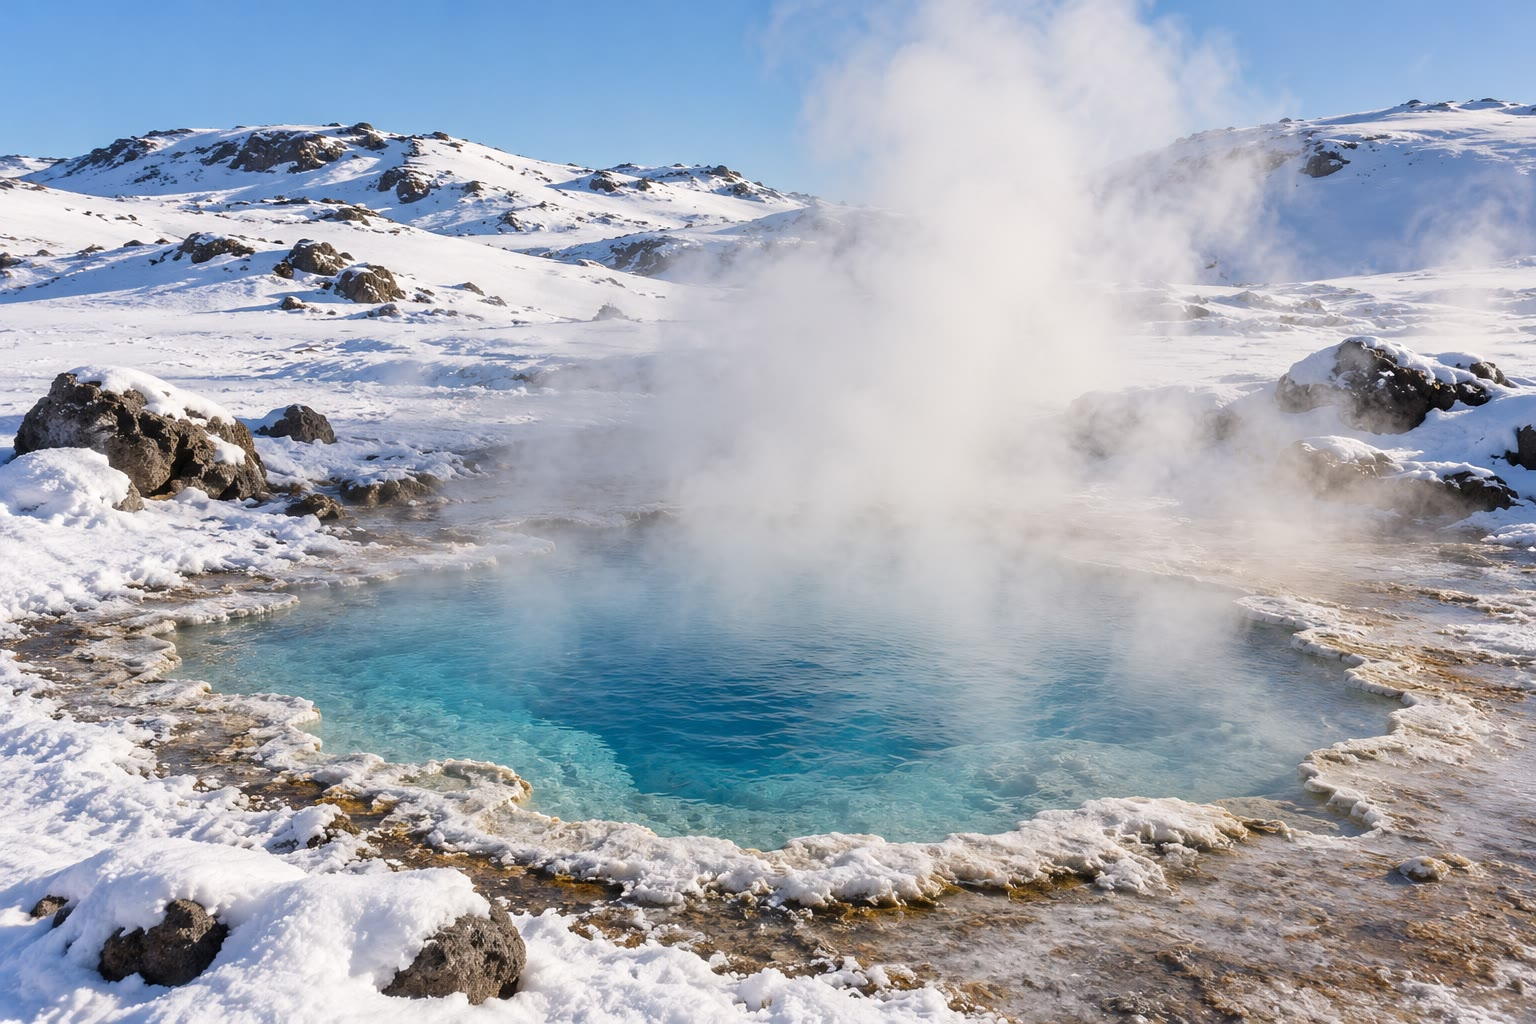
\includegraphics[width=0.6\linewidth]{images/book2/ai/g12-hot-spring-snow.jpg}

{\small बर्फ़ीले भूदृश्य में भाप छोड़ता एक गरम सोता: गहरे भूमिगत गरम हुआ जल
सतह पर लौट आता है। एआई-जनित चित्रण।}
\end{omfigure}

\begin{omfigure}
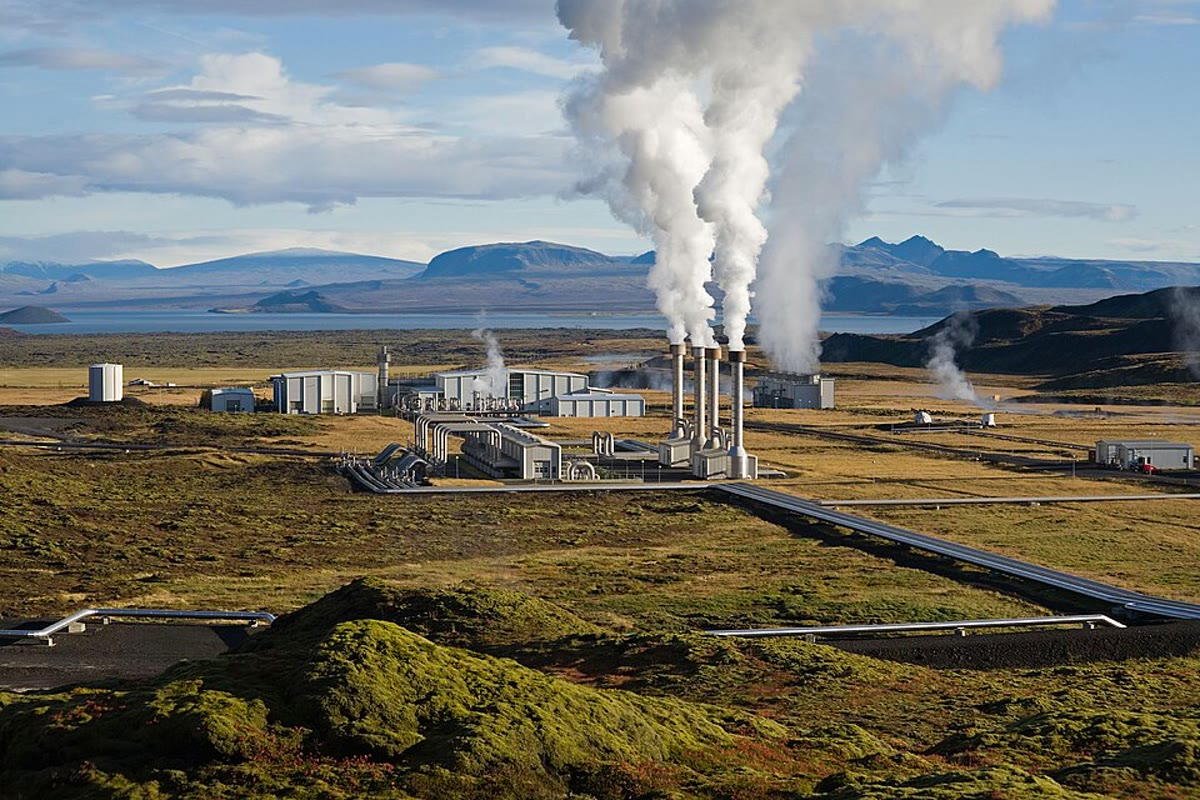
\includegraphics[width=0.66\linewidth]{images/book2/g12-nesjavellir-geothermal.jpg}

{\small आइसलैंड के ज्वालामुखीय हेंगिल क्षेत्र में नेस्यावेटलिर भूतापीय
बिजलीघर: \qty{120}{MW} तक बिजली और
\qty{300}{MW} तक ऊष्मा, गरम जल द्वारा ले जाई गई। फ़ोटो ग्रेटार
ईवार्सन (सार्वजनिक डोमेन)।}
\end{omfigure}
% ledger: photo:g12-nesjavellir, on:nesjavellir

कोई भूतापीय क्षेत्र मानव जीवन के पैमाने पर अक्षय नहीं है। कैलिफ़ोर्निया के
गीज़र्स क्षेत्र में बहुत अधिक कुओं ने भाप खींची, उससे तेज़ी से जितनी तेज़ी से
धीमा \omterm{def:g12:internal-heat:heat-flow}{ऊष्मा-प्रवाह} और वर्षा उसकी पूर्ति कर सकते थे: भाप का दाब अपने चरम के आधे से भी
कम हो गया, और बिजलीघरों की \qty{40}{\percent} से अधिक
क्षमता खो गई। गिरावट को धीमा करने के लिए अब जल वापस
क्षेत्र में डाला जाता है।
% ledger: cpuc:geysers

\section{अभ्यास}

\begin{exercise}[$\star$]\label{exo:g12:internal-heat:1}
शब्द बताइए: (a) सतह के हर वर्ग मीटर से होकर भीतरी भाग से निकलने वाली
शक्ति; (b) चट्टान के एकक आयतन में रेडियोधर्मी परमाणुओं के क्षय से मुक्त
ऊष्मा; (c) पृथ्वी के बनने के समय से संचित ऊष्मा की हानि;
(d) स्वयं पदार्थ की गति द्वारा ऊष्मा का परिवहन; (e) पृथ्वी की
आंतरिक ऊष्मा जिसका उपयोग लोग करते हैं।
\end{exercise}

\begin{exercise}[$\star$]\label{exo:g12:internal-heat:2}
बदलिए: (1) \qty{91.6}{mW/m^2} को \unit{W/m^2} में; (2) \qty{46.7}{TW} को
वाट में; (3) प्रति किलोमीटर \qty{29}{\celsius} को केल्विन प्रति मीटर में।
\end{exercise}

\begin{exercise}[$\star$]\label{exo:g12:internal-heat:3}
उन चार समस्थानिकों के नाम बताइए जो लगभग सारी रेडियोजनित ऊष्मा बनाते हैं, और बताइए कि
कमलैंड संसूचक उनमें से कौन-से दो देख सकता है।
\end{exercise}

\begin{exercise}[$\star$]\label{exo:g12:internal-heat:4}
$q = 490/\sqrt{t}$ का उपयोग करके 1, 4,
25 और 49 मिलियन वर्ष पुरानी महासागरीय तली से होकर \omterm{def:g12:internal-heat:heat-flow}{ऊष्मा-प्रवाह} परिकलित कीजिए।
\end{exercise}

\begin{exercise}[$\star$]\label{exo:g12:internal-heat:5}
\omterm{def:g12:internal-heat:heat-flow}{ऊष्मा-प्रवाह} को सतह पर ही मापने के बजाय बोरछिद्रों में क्यों मापा जाता है?
खोदने के बाद मापने से पहले प्रतीक्षा क्यों करनी चाहिए?
\end{exercise}

\begin{exercise}[$\star\star$]\label{exo:g12:internal-heat:6}
केटीबी बोरछिद्र में \qty{9.1}{km} पर चट्टान लगभग \qty{265}{\celsius} पर
थी। (1) सतह पर \qty{10}{\celsius} मानकर माध्य
प्रवणता परिकलित कीजिए। (2) \qty{2.72}{W/(m.K)} की चालकता के साथ यह कितना \omterm{def:g12:internal-heat:heat-flow}{ऊष्मा-प्रवाह}
देती है? (3) महाद्वीपों के माध्य से तुलना कीजिए।
\end{exercise}

\begin{exercise}[$\star\star$]\label{exo:g12:internal-heat:7}
महाद्वीप \qty{70.9}{mW/m^2} के माध्य \omterm{def:g12:internal-heat:heat-flow}{ऊष्मा-प्रवाह} के साथ \qty{2.073e14}{m^2} ढकते हैं,
महासागर \qty{105.4}{mW/m^2} के साथ \qty{3.028e14}{m^2}। हर एक द्वारा खोई गई शक्ति,
कुल, और महासागरीय तली से खोया गया
अंश परिकलित कीजिए।
\end{exercise}

\begin{exercise}[$\star\star$]\label{exo:g12:internal-heat:8}
\qty{8}{km} मोटी \omterm{def:g12:subduction-magmatism:granodiorite}{ग्रैनोडायोराइट} की एक परत का ऊष्मा-उत्पादन
\qty{1.88}{\micro W/m^3} है। (1) वह सतह पर कितना \omterm{def:g12:internal-heat:heat-flow}{ऊष्मा-प्रवाह} उत्पन्न करती है?
(2) यह \qty{70.9}{mW/m^2} का कितना अंश है?
\end{exercise}

\begin{exercise}[$\star\star$]\label{exo:g12:internal-heat:9}
$q = 490/\sqrt{t}$ के अनुसार, किस आयु पर महासागरीय तली उतनी ऊष्मा खोती है जितनी औसत महाद्वीप,
\qty{70.9}{mW/m^2}?
\end{exercise}

\begin{exercise}[$\star\star$]\label{exo:g12:internal-heat:10}
1.4 अरब वर्ष पहले यूरेनियम-235 ने आज की अपेक्षा कितने गुना अधिक ऊष्मा मुक्त की?
और 2.5 अरब वर्ष पहले पोटैशियम-40 ने?
\end{exercise}

\begin{exercise}[$\star\star$]\label{exo:g12:internal-heat:11}
$t \approx L^2/\kappa$ का उपयोग करके, $\kappa = \qty{1e-6}{m^2/s}$ के साथ, बताइए कि
चालन द्वारा ऊष्मा को पार करने में कितना समय लगता है: (1) \qty{10}{m} मोटा एक लावा-प्रवाह;
(2) \qty{100}{km} मोटा \omterm{def:g11:lithosphere-asthenosphere:lithosphere}{स्थलमंडल}; (3) प्रावार? हर परिणाम को
उचित इकाइयों में व्यक्त कीजिए।
\end{exercise}

\begin{exercise}[$\star\star\star$]\label{exo:g12:internal-heat:12}
आज थोरियम-232 लगभग \qty{10.4}{TW}, यूरेनियम-238 \qty{9.6}{TW},
पोटैशियम-40 \qty{4.0}{TW} और यूरेनियम-235 \qty{0.42}{TW} मुक्त करते हैं। चित्र की
अर्ध-आयुओं का उपयोग करके, 3 अरब वर्ष पहले हर एक की ऊष्मा,
कुल, और दोनों अल्पायु
समस्थानिकों का अंश परिकलित कीजिए।
\end{exercise}

\begin{exercise}[$\star\star\star$]\label{exo:g12:internal-heat:13}
नेस्यावेटलिर बिजलीघर \qty{300}{MW} तक ऊष्मा दे सकता है,
जिसे प्रति सेकंड लगभग \qty{1640}{L} गरम जल ढोता है। \qty{4180}{J/(kg.K)} की विशिष्ट ऊष्मा
और प्रति लीटर \qty{1}{kg} द्रव्यमान के साथ, यह जल कितने
अंश गरम हुआ है? औसत महाद्वीप का कितना बड़ा क्षेत्रफल
\qty{300}{MW} ऊष्मा खोता है?
\end{exercise}

\begin{exercise}[$\star\star\star$]\label{exo:g12:internal-heat:14}
मान लीजिए किसी प्लेट को कटक से खाई तक जाने में 100 मिलियन वर्ष लगते हैं, और
पूरे प्रावार से होकर संवहन के एक लूप को लगभग 200 मिलियन वर्ष। (1)
इन समयों की तुलना प्रावार के आर-पार चालन के 260 अरब वर्षों से कीजिए।
(2) संवहन ऊष्मा को इतनी अधिक तेज़ी से क्यों ले जा सकता है, यद्यपि
प्रावार प्रति वर्ष केवल कुछ सेंटीमीटर चलता है?
\end{exercise}

\begin{exercise}[$\star\star\star$]\label{exo:g12:internal-heat:15}
मान लीजिए क्रोड \qty{2891}{km} नीचे, \omterm{def:g11:seismic-structure:core}{क्रोड--प्रावार सीमा} के आर-पार, प्रावार में
लगभग \qty{10}{TW} ऊष्मा खोता है। (1) यह \qty{22.3}{TW} के
\omterm{def:g12:internal-heat:secular-cooling}{दीर्घकालिक शीतलन} का कितना अंश होगा? शेष कहाँ से
आता है? (2) \omterm{def:g11:seismic-structure:core}{क्रोड--प्रावार सीमा} के आर-पार माध्य \omterm{def:g12:internal-heat:heat-flow}{ऊष्मा-प्रवाह} परिकलित कीजिए,
और उसकी तुलना सतह पर के माध्य \omterm{def:g12:internal-heat:heat-flow}{ऊष्मा-प्रवाह},
\qty{91.6}{mW/m^2}, से कीजिए। (3) प्रावार के ठोस होते हुए भी गरम क्रोड
प्रावार के आधार को क्यों गरम कर सकता है?
\end{exercise}

\begin{problem}[{सप्ताहांत समस्या --- पृथ्वी का ऊष्मा-बजट}]
\label{pb:g12:internal-heat:1}
% ledger: b2dd10:continents, b2dd10:half-space, kamland11:geonu, dye12:isotopes, dye12:bse, b2vila:heat-production
% values (internal_heat.py): radiogenic 24.4 TW, secular 22.3 TW, share 0.523, K40 4.0, U235 0.42, U238 9.59
पृथ्वी का \omterm{def:g12:internal-heat:heat-flow}{ऊष्मा-प्रवाह} 38\,000 से अधिक स्थानों पर मापा गया है।
औसतन महाद्वीप \qty{2.073e14}{m^2} पर \qty{70.9}{mW/m^2} खोते हैं,
और महासागरीय तली \qty{3.028e14}{m^2} पर \qty{105.4}{mW/m^2}।

\medskip
\noindent\textbf{भाग I --- ऊष्मा-प्रवाह और क्षेत्रफल।}
\begin{enumerate}
  \item जाँचिए कि दोनों क्षेत्रफल जुड़कर \qty{6371}{km} त्रिज्या वाले गोले के
        क्षेत्रफल के बराबर होते हैं।
  \item सतह का कितना अंश महासागरीय तली है?
  \item महासागरीय तली प्रति वर्ग मीटर महाद्वीपों से अधिक ऊष्मा
        क्यों खोती है?
  \item $q = 490/\sqrt{t}$ का उपयोग करके 4 मिलियन वर्ष पुरानी
        महासागरीय तली से होकर \omterm{def:g12:internal-heat:heat-flow}{ऊष्मा-प्रवाह} परिकलित कीजिए।
  \item ग्रेनाइट (\qty{2.72}{W/(m.K)}) में एक बोरछिद्र प्रति किलोमीटर
        \qty{26}{\celsius} मापता है। उसका \omterm{def:g12:internal-heat:heat-flow}{ऊष्मा-प्रवाह} महाद्वीपीय माध्य से
        ऊपर है या नीचे?
\end{enumerate}

\medskip
\noindent\textbf{भाग II --- कुल।}
\begin{enumerate}[resume]
  \item महाद्वीपों से होकर खोई गई शक्ति परिकलित कीजिए।
  \item महासागरीय तली से होकर खोई गई शक्ति परिकलित कीजिए।
  \item उन्हें जोड़िए: पृथ्वी का कुल \omterm{def:g12:internal-heat:heat-flow}{ऊष्मा-प्रवाह}, टेरावाट में।
  \item पूरी सतह पर माध्य \omterm{def:g12:internal-heat:heat-flow}{ऊष्मा-प्रवाह} क्या है?
  \item यदि हर महाद्वीप के नीचे \qty{10}{km} ग्रेनाइट (\qty{24.3}{mW/m^2}) होता,
        तो वह कितने टेरावाट उत्पन्न करता? इसकी तुलना
        महाद्वीपों से होकर खोई गई शक्ति से कीजिए।
\end{enumerate}

\medskip
\noindent\textbf{भाग III --- रेडियोजनित ऊष्मा।}
\begin{enumerate}[resume]
  \item कमलैंड यूरेनियम-238 और थोरियम-232 के भू-न्यूट्रिनो गिनता है: मिलकर
        वे लगभग \qty{20.0}{TW} मुक्त करते हैं, पृथ्वी में यूरेनियम के हर किलोग्राम के लिए
        \qty{3.9}{kg} थोरियम के साथ। एक किलोग्राम यूरेनियम अपने यूरेनियम-238 से
        \qty{94.4}{\micro W} और अपने यूरेनियम-235 से \qty{4.10}{\micro W}
        मुक्त करता है; एक किलोग्राम थोरियम, \qty{26.3}{\micro W}।
        पहले यूरेनियम-238 की ऊष्मा परिकलित कीजिए, फिर यूरेनियम-235 की।
  \item पोटैशियम-40 लगभग \qty{4}{TW} जोड़ता है। कुल रेडियोजनित ऊष्मा परिकलित कीजिए।
  \item किस प्रकार की चट्टान इन तत्त्वों का अधिकांश भाग रखती है, और वह कहाँ है?
  \item 3 अरब वर्ष पहले रेडियोजनित ऊष्मा अधिक थी या कम? क्यों?
\end{enumerate}

\medskip
\noindent\textbf{भाग IV --- दीर्घकालिक शीतलन।}
\begin{enumerate}[resume]
  \item कितनी शक्ति की पूर्ति रेडियोधर्मिता नहीं करती?
  \item वह कहाँ से आती है?
  \item \omterm{def:g12:internal-heat:heat-flow}{ऊष्मा-प्रवाह} का वह अंश परिकलित कीजिए जिसकी पूर्ति \omterm{def:g12:internal-heat:secular-cooling}{दीर्घकालिक शीतलन} करता है।
  \item पृथ्वी के संघटन के मॉडल 11 से
        \qty{38}{TW} की रेडियोजनित ऊष्मा देते हैं।
        तब रेडियोजनित भाग किन अंशों के बीच पड़ता है?
  \item प्रावार से होकर इस ऊष्मा का अधिकांश भाग कौन ले जाता है?
  \item सारांश दीजिए: आज पृथ्वी की ऊष्मा-हानि का कितना अंश रेडियोधर्मिता
        देती है?
\end{enumerate}
\end{problem}
